%% main.tex — IEEE Conference Format
%% Based on IEEEtran.cls (conference mode)

\documentclass[conference]{IEEEtran}
\IEEEoverridecommandlockouts

% ── Core packages ──────────────────────────────────────────────────────────────
\usepackage{cite}
\usepackage{amsmath,amssymb,amsfonts}
\usepackage{algorithmic}
\usepackage{graphicx}
\usepackage{textcomp}
\usepackage{xcolor}
\usepackage{multirow}
\usepackage{array}
\usepackage{rotating}
\usepackage{float}
\usepackage{tikz}
\usetikzlibrary{shapes.geometric, arrows, arrows.meta, positioning, trees, fit, backgrounds}

% ── Custom centred fixed-width column ──────────────────────────────────────────
\newcolumntype{C}[1]{>{\centering\arraybackslash}p{#1}}


\def\BibTeX{{\rm B\kern-.05em{\sc i\kern-.025em b}\kern-.08em
    T\kern-.1667em\lower.7ex\hbox{E}\kern-.125emX}}

% ══════════════════════════════════════════════════════════════════════════════
\begin{document}

\title{ABR Streaming Algorithms: A Comparative Study\\ of Buffer-Centric and Throughput-Based}

\author{%
  \IEEEauthorblockN{Nguyen N.T. Nhung}
  \IEEEauthorblockA{%
    \textit{Digital Communication and Multimedia Engineer\\SEEE, HUST}\\
    \textit{}
    Student ID: 202414652\\
    nhung.nth2414652@sis.hust.edu.vn}
}

\maketitle

% ── Abstract ──────────────────────────────────────────────────────────────────
\begin{abstract}
Adaptive bitrate (ABR) streaming algorithms must balance video quality
against the risk of playback interruption under variable network conditions.
This paper presents a comparative study of two ABR control strategies
implemented within a discrete-event simulation (DES) framework: a Predictive
Throughput Controller based on harmonic-mean bandwidth estimation, and the
Lyapunov Buffer Controller (BOLA), which maximizes a logarithmic utility
function subject to playback buffer occupancy constraints.  Both controllers
are evaluated across nine benchmark scenarios covering stable WiFi,
constrained 3G mobile, high-frequency oscillation, and manifest stress
conditions.  Results show that BOLA consistently outperforms the Predictive
Controller in stable and bandwidth-constrained environments, achieving up
to 95\% higher QoE at tier-boundary operating points, while the Predictive
Controller is more robust during abrupt bandwidth collapses.  These
complementary failure modes motivate a hybrid design that combines
throughput estimation during transient phases with Lyapunov optimization
at steady state.
\end{abstract}

\begin{IEEEkeywords}
adaptive bitrate streaming, MPEG-DASH, BOLA, Lyapunov optimization,
quality of experience, buffer-based adaptation
\end{IEEEkeywords}

% ══════════════════════════════════════════════════════════════════════════════
\section{Introduction}
In contemporary telecommunication infrastructures, internet video streaming has evolved from a premium application modality into the dominant consumer of global network traffic, currently accounting for over 80\% of aggregate data payloads. This unprecedented surge in multimedia data transfer has fundamentally exposed the architectural limitations of classical transport systems. Historically, streaming service providers relied on stateful, continuous streaming protocols or progressive HTTP downloads, delivering a single monolithic media container sequentially over a traditional TCP connection. This static paradigm is highly fragile when deployed over wireless modern channels; any sudden plunge in localized channel capacity causes immediate packet delivery delay, forcing the client playout queue to starve, which results in disruptive playout freezes or long initial loading delays.

To resolve these transport vulnerabilities, the industry underwent a structural paradigm shift toward HTTP-based adaptive streaming, primarily standardized under the \textbf{Dynamic Adaptive Streaming over HTTP (MPEG-DASH)} framework \cite{iso23009}. Under MPEG-DASH, source video streams are statically partitioned at the server architecture into brief, self-contained temporal slices known as segments or chunks, usually ranging from 2 to 10 seconds in length. Each spatial-temporal segment is pre-encoded and cached across a multi-tier resolution and bitrate matrix. By shifting the control intelligence entirely to the client application layer, MPEG-DASH leverages standard, stateless HTTP infrastructure and Content Delivery Networks (CDNs) \cite{jiang2012}. The client playback engine can adapt quality profiles dynamically on a chunk-by-chunk basis, pulling the most appropriate bitrate profile from the server repository depending on real-time environmental observations.

The execution of any Adaptive Bitrate (ABR) rate adaptor is governed by a multi-objective optimization problem that must manage an inherent, zero-sum trade-off in network multimedia delivery:
\begin{itemize}
    \item \textbf{Perceptual Quality Maximization:} The client engine aims to request the highest possible bitrate representation from the server matrix to saturate available channel pipes. Superior bitrates correspond directly to high pixel fidelity, sharp spatial resolutions, and minimal codec compression artifacts, directly maximizing user satisfaction.
    \item \textbf{Playout Starvation Minimization:} Concurrently, the algorithm must maintain a conservative safety guard band to defend the playback pipeline against underflow hazards. If the transmission download latency of an assigned segment exceeds the residual playback time buffered in client memory, the movie screen freezes, triggering a catastrophic rebuffering or stalling event.
\end{itemize}
Because wireless cellular channel capacities are highly non-stationary, stochastic, and unpredictable, aggressive quality upgrades risk immediate buffer depletion, whereas overly cautious rate requests sacrifice visual quality by streaming pixelated low-resolution payloads \cite{spiteri2020}.

To manage this trade-off, two competing rate-adaptation philosophies have emerged in core research literature. The first category comprises heuristic \textbf{Throughput-Based Algorithms} (e.g., the FESTIVE framework) \cite{jiang2012}. These controllers estimate future network capacities by applying sliding window smoothing filters, such as the Harmonic Mean, onto historical segment download transfer logs. While effective at tracking macro-network trends, throughput-based prediction models are highly sensitive to sudden channel fluctuations or application-layer reporting noise. The second category features control-theoretic \textbf{Buffer-Based Controllers}, led by the Near-Optimal BOLA framework \cite{spiteri2020}. Grounded in Michael Neely’s Lyapunov Drift-Plus-Penalty control theory \cite{neely2010}, BOLA circumvents the instability of bandwidth forecasting entirely by making decisions based solely on instantaneous buffer occupancy states $Q(t)$, guaranteeing asymptotic time-average utility maximization.

To conduct a systematic evaluation of these control mechanisms without the system noise of live over-the-air cell traffic, this project designs and deploys a rigorous, object-oriented \emph{Discrete-Event Simulation (DES)} platform implemented via Python and visual declarative front-ends. The primary contributions of this work are three-fold:
\begin{enumerate}
    \item We construct an isolated three-zone multimedia testing framework that simulates VBR server encoding variances, stochastic network interpolated channel drops, round-trip propagation costs, and real-time client playout buffer dynamics.
    \item We implement an advanced, engineered hybrid rate arbitrator that implements a predictive heuristic phase to bootstrap playout memory during cold-start intervals, mitigating the startup latency vulnerabilities of pure buffer-based controllers.
    \item We cross-examine the controllers across nine distinct benchmark scenarios—ranging from stable high-speed configurations to constrained mobile channels—and analyze a critical corner-case anomaly where network logging noise reveals BOLA's mathematical resilience over predictive filters.
\end{enumerate}

The remainder of this technical report is organized as follows: Section~II reviews the core background of MPEG-DASH architectures, predictive harmonic filters, and Lyapunov optimization mechanics. Section~III maps out the detailed 10-block discrete simulation architecture and data-routing dependencies. Section~IV specifies the mathematical formulation of our algorithms and hybrid control loop extensions. Section~V details the software engineering deployment stack and input asset configurations. Finally, Section~VI and Section~VII present the objective evaluation metrics, benchmark scorecards, and a deep-dive critical analysis of empirical results.

\section{Background \& Related Work}

\subsection{MPEG-DASH System Architecture}

Dynamic Adaptive Streaming over HTTP (MPEG-DASH), standardized under
ISO/IEC~23009-1~\cite{iso23009}, establishes a universal framework for
streaming multimedia data across unmanaged, heterogeneous IP networks.
Unlike traditional stateful streaming protocols that require dedicated
network-layer infrastructure, MPEG-DASH relies entirely on the ubiquitous
and stateless HTTP/TCP paradigm.  By offloading session tracking and
delivery logic from media servers to client application layers, the system
achieves high scalability, network resilience, and seamless compatibility
with standard Content Delivery Networks (CDNs) and proxy
caches~\cite{jiang2012}.

The core mechanism of MPEG-DASH is a client-driven pull architecture.
Multimedia content is organized using an XML index called the
\emph{Media Presentation Description} (MPD), or manifest
file~\cite{iso23009}.  The hierarchical structure is shown in
Fig.~\ref{fig:mpd_hierarchy}.

\begin{figure}[t]
\centering
\begin{tikzpicture}[
    edge from parent fork down,
    level distance=1.5cm,
    growth direction=south,
    sibling distance=4.5cm,
    every node/.style={draw, rectangle, rounded corners, fill=blue!5,
      text width=4.2cm, align=center, font=\scriptsize}
]
\node {Media Presentation Description\\(MPD Manifest File)}
    child {node {Period\\(Scene / Temporal Interval)}
        child {node {AdaptationSet\\(Media Type: Video / Audio)}
            child {node {Representation~0\\(360p, 500\,kbps)\\Chunks: $S_{k,0}$}}
            child {node {Representation~$M{-}1$\\(1080p, 5\,Mbps)\\Chunks: $S_{k,M-1}$}}
        }
    };
\end{tikzpicture}
\caption{Hierarchical structure of the MPEG-DASH MPD.}
\label{fig:mpd_hierarchy}
\end{figure}

As shown in Fig.~\ref{fig:mpd_hierarchy}, an MPD contains one or more
sequential Periods, each holding AdaptationSets for each media type.
Each AdaptationSet offers multiple Representations---encodings of the same
content at different bitrates---divided into fixed-duration
Segments~\cite{spiteri2020}.

\subsubsection{Mathematical Abstraction of Server Multimedia Data}

Let $\mathcal{M}=\{0,1,\dots,M{-}1\}$ denote the set of available quality
representations.  Each tier $m\in\mathcal{M}$ maps to a nominal encoding
bitrate:
\begin{equation}
  \mathcal{R}=\{R_0,R_1,\dots,R_{M-1}\}, \quad R_0<R_1<\cdots<R_{M-1}.
\end{equation}

Every segment $k\in\{0,1,\dots,N{-}1\}$ has a fixed playout duration~$p$
(seconds).  To model Variable Bitrate (VBR) encoding, the file size
$S_{k,m}$ (in bytes) is drawn stochastically:
\begin{equation}
  \tilde{S}_{k,m}\sim\mathcal{N}(\mu_m,\,\sigma_m^2),\quad
  \mu_m=\frac{R_m\cdot p}{8},
\end{equation}
with $\sigma_m=0.20\,\mu_m$ and a hard floor preventing non-positive values:
\begin{equation}
  S_{k,m}=\max\!\left(\tilde{S}_{k,m},\;0.10\,\mu_m\right).
\end{equation}

% ──────────────────────────────────────────────────────────────────────────────
\subsection{Heuristic Throughput-Based Approaches}

\subsubsection{Predictive Bandwidth Estimation}

Throughput-based algorithms select the next bitrate tier based on recent
download measurements.  A well-known example is the FESTIVE
framework~\cite{jiang2012}, which assumes short-term capacity correlates
with past throughput samples.

Raw wireless measurements fluctuate due to cross-traffic, handovers, and
TCP dynamics.  A plain arithmetic mean tends to overestimate capacity,
causing the client to request a higher tier than the network can sustain.

\subsubsection{Harmonic Mean Filter}

To reduce sensitivity to outliers, a harmonic mean filter is applied over
a sliding window of the last $W=5$ download rates
$\mathcal{H}_k=\{\omega_{k-W+1},\dots,\omega_k\}$:
\begin{equation}
  \hat{\omega}_{k+1}=\frac{W}{\displaystyle\sum_{i=0}^{W-1}
    \dfrac{1}{\max(\omega_{k-i},\,1.0)}}.
  \label{eq:harmonic_mean}
\end{equation}

The $\max(\cdot,1.0)$ floor prevents division-by-zero during channel
blackouts.  Because the harmonic mean is sensitive to small values, a single
stalled segment heavily penalizes the estimate, yielding a conservative and
safe bandwidth prediction.

\subsubsection{Safety Margin and Rate Selection}

A safety coefficient $\rho\in(0,1]$ (set to $\rho=0.9$) produces the
sustainable throughput threshold:
\begin{equation}
  \omega_{\text{safe}}=\hat{\omega}_{k+1}\times\rho.
  \label{eq:safe_throughput}
\end{equation}

The client selects the highest quality tier satisfying the capacity
constraint:
\begin{equation}
  m^*=\max\!\left\{m\in\mathcal{M}\mid R_m\le\omega_{\text{safe}}\right\}.
  \label{eq:throughput_selection}
\end{equation}

If $\omega_{\text{safe}}<R_0$ or $\mathcal{H}_k=\emptyset$, the algorithm
defaults to $m^*=0$.  The complete procedure is summarized in
Algorithm~\ref{alg:throughput_abr}.

\begin{figure}[htbp]
\renewcommand{\arraystretch}{1.2}
\centering
\begin{tabular}{p{0.88\columnwidth}}
\hline
\textbf{Algorithm~1: Heuristic Throughput-Based Rate Adaptation}\\
\hline
\textbf{Input:} History queue $\mathcal{H}_k$, bitrate set $\mathcal{R}$,
  safety margin $\rho$\\
\textbf{Output:} Quality index $m^*$\\
1:~\textbf{if} $\mathcal{H}_k=\emptyset$ \textbf{then return} $0$\\
2:~$\mathit{SumRec}\leftarrow 0$\\
3:~\textbf{for} each $\omega$ in last $W$ entries of $\mathcal{H}_k$
  \textbf{do}\\
4:~\quad$\mathit{SumRec}\leftarrow\mathit{SumRec}+1/\max(\omega,1.0)$\\
5:~\textbf{end for}\\
6:~$\hat{\omega}_{k+1}\leftarrow W/\mathit{SumRec}$\\
7:~$\omega_{\text{safe}}\leftarrow\hat{\omega}_{k+1}\times\rho$\\
8:~$m^*\leftarrow 0$\\
9:~\textbf{for} $m=M{-}1$ \textbf{down to} $0$ \textbf{do}\\
10:~\quad\textbf{if} $R_m\le\omega_{\text{safe}}$ \textbf{then}\\
11:~\qquad$m^*\leftarrow m$;~\textbf{break}\\
12:~\quad\textbf{end if}\\
13:~\textbf{end for}\\
14:~\textbf{return} $m^*$\\
\hline
\end{tabular}
\caption{Playout adaptation logic based on historic channel state indicators.}
\label{alg:throughput_abr}
\end{figure}

% ──────────────────────────────────────────────────────────────────────────────
\subsection{Buffer-Based Control and Stochastic Optimization}

\subsubsection{Limitations of Throughput-Based Adaptation}

Throughput-based controllers try to solve an application-layer problem
using noisy network-layer estimates.  Buffer-based controllers instead use
the client playout buffer occupancy $Q(t)$, which acts as a smoothed
proxy for network health.  The problem becomes: keep $Q(t)$ within a safe
range while maximizing video quality~\cite{spiteri2020}.

\subsubsection{Lyapunov Drift Theory}
The buffer-based controller is grounded in the Lyapunov drift-plus-penalty framework for stochastic systems~\cite{neely2010}.  Define the quadratic Lyapunov function:
\begin{equation}
  L(Q(t)) = \frac{1}{2}\left[Q(t) - Q_{\max}\right]^2,
  \label{eq:lyapunov}
\end{equation}
and the conditional one-step drift:
\begin{equation}
  \Delta L(Q(t)) \triangleq \mathbb{E}\!\left\{L(Q(t{+}1)) - L(Q(t)) \mid Q(t)\right\}.
  \label{eq:drift}
\end{equation}

To maximize user quality satisfaction while bounding underflow risk, the controller minimizes the unified drift-plus-penalty objective bound~\cite{neely2010}:
\begin{equation}
  \min \; \Delta L(Q(t)) - V \cdot \mathbb{E}\!\left\{v_m \mid Q(t)\right\},
  \label{eq:dpp}
\end{equation}
where $v_m$ is the perceptual utility of representation~$m$ and $V>0$ trades off quality utility optimization against physical buffer safety requirements.

\subsubsection{The BOLA Optimization Objective}

Expanding the drift bound and isolating the controllable decision variable,
Spiteri et al.~\cite{spiteri2020} derive a closed-form real-time control
law.  At each segment download event, the client selects:
\begin{equation}
  m^*=\operatorname*{arg\,max}_{m\in\mathcal{M}}
    \frac{V\cdot(v_m+\gamma)-\left[Q(t)-\tau\right]}{S_{k,m}},
  \label{eq:bola_objective}
\end{equation}
where $v_m=\ln(R_m/R_0)$ is the logarithmic perceptual utility,
$\tau$ is a buffer safety offset, and $\gamma$ stabilizes quality
transitions.

Because \eqref{eq:bola_objective} depends only on $S_{k,m}$ and $Q(t)$,
it runs at $\mathcal{O}(M)$ complexity and bounds time-average performance
to within $\mathcal{O}(1/V)$ of the theoretical
optimum~\cite{spiteri2020,neely2010}.  Algorithm~\ref{alg:bola_abr}
formalizes the procedure.

\begin{figure}[htbp]
\renewcommand{\arraystretch}{1.2}
\centering
\begin{tabular}{p{0.88\columnwidth}}
\hline
\textbf{Algorithm~2: Lyapunov-Optimized Rate Adaptation (BOLA)}\\
\hline
\textbf{Input:} Buffer level $Q(t)$, offset $\tau$, parameters $V,\gamma$,
  segment sizes $\{S_{k,m}\}$, utilities $\{v_m\}$\\
\textbf{Output:} Quality index $m^*$\\
1:~\textbf{if} $Q(t)\le\tau$ \textbf{then return} $0$\\
2:~$\mathit{MaxObj}\leftarrow-\infty$;~$m^*\leftarrow 0$\\
3:~\textbf{for} $m=0$ \textbf{to} $M{-}1$ \textbf{do}\\
4:~\quad$\mathit{sz}\leftarrow\max(S_{k,m},1.0)$\\
5:~\quad$\mathit{Obj}\leftarrow\bigl[V(v_m+\gamma)-(Q(t)-\tau)\bigr]/\mathit{sz}$\\
6:~\quad\textbf{if} $\mathit{Obj}>\mathit{MaxObj}$ \textbf{then}\\
7:~\qquad$\mathit{MaxObj}\leftarrow\mathit{Obj}$;~$m^*\leftarrow m$\\
8:~\quad\textbf{end if}\\
9:~\textbf{end for}\\
10:~\textbf{return} $m^*$\\
\hline
\end{tabular}
\caption{Lyapunov drift minimization loop for real-time buffer-safety optimization.}
\label{alg:bola_abr}
\end{figure}

% ══════════════════════════════════════════════════════════════════════════════
\section{System Design \& Architecture}

\subsection{Modular Architecture}

The framework uses a Discrete-Event Simulation (DES) architecture where the
virtual clock jumps between segment download events, ensuring full
reproducibility and isolation of adaptation logic from environmental
variables.

The design is split into three functional zones:
\begin{itemize}
  \item Zone~1 (Server Abstraction): a stateless module storing the MPD
    structure and VBR segment sizes.
  \item Zone~2 (Network Channel): applies trace-driven bandwidth profiles,
    jitter, and RTT delays.
  \item Zone~3 (Adaptive Client Engine): contains the buffer manager, ABR
    controllers, telemetry logger, and visualization dashboard.
\end{itemize}

\subsection{The 10-Block Event-Driven Pipeline}

The runtime execution loop is decomposed into ten functional blocks,
co-operating via localized state-change boundaries as shown in
Fig.~\ref{fig:10_block_pipeline}.

% ── Fig. 4: 10-Block Pipeline — labels inside zones, no overlap, dark palette
\begin{figure}[htbp]
\centering
\resizebox{0.97\columnwidth}{!}{%
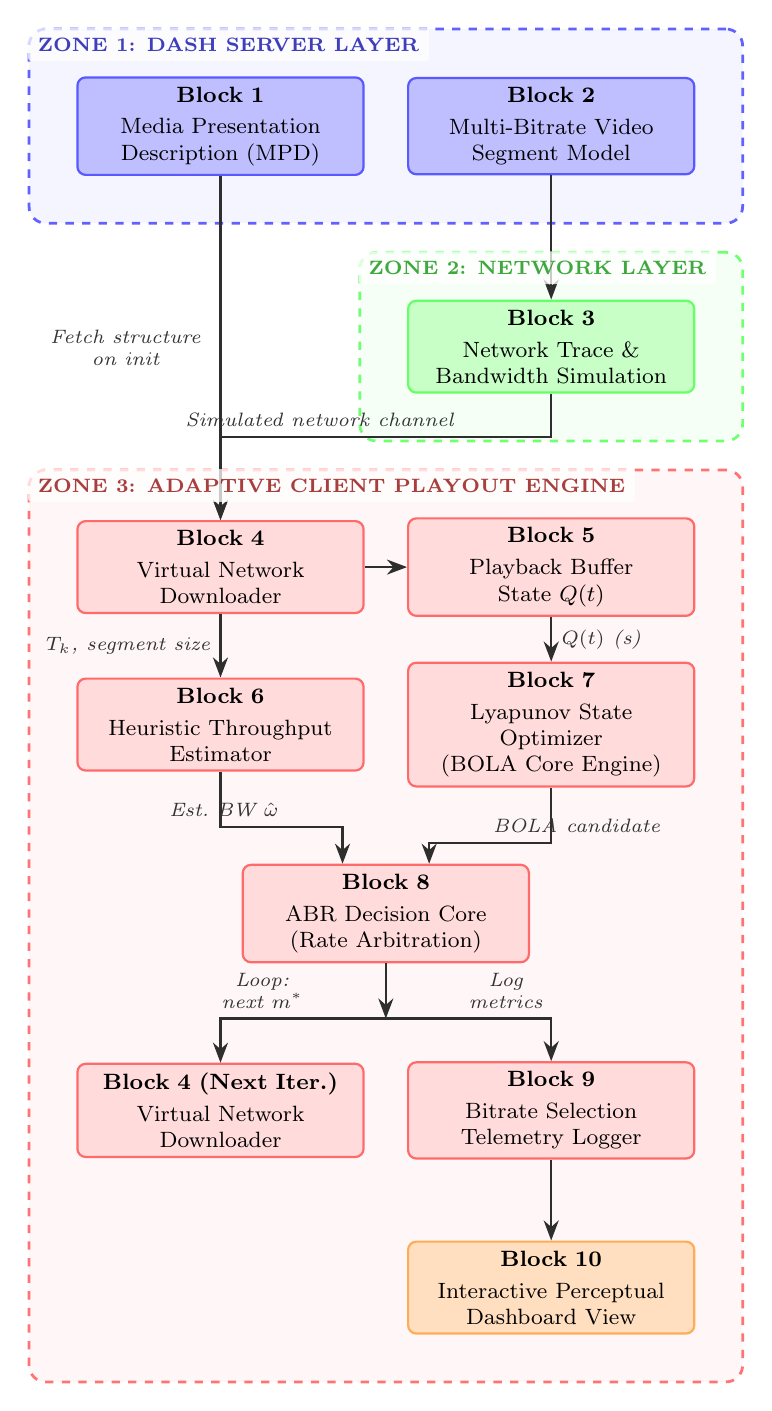
\begin{tikzpicture}[
    % ── Block node style ─────────────────────────────────────────────
    block/.style={
        draw, rectangle, rounded corners=3pt,
        minimum height=1.1cm, text width=3.4cm,
        align=center, font=\footnotesize, line width=0.8pt
    },
    % ── Block fill colours (darker, moderate contrast) ────────────────
    zone1/.style={fill=blue!25,   draw=blue!65},
    zone2/.style={fill=green!22,  draw=green!60},
    zone3/.style={fill=red!14,    draw=red!58},
    zone4/.style={fill=orange!25, draw=orange!65},
    % ── Arrows: solid black ──────────────────────────────────────────
    arrow/.style={thick, -{Stealth[scale=1.1]}, draw=black!82},
    % ── Edge labels: dark, small, italic ─────────────────────────────
    lbl/.style={font=\scriptsize\itshape, align=center, text=black!80},
    % ── Zone container: dashed border, generous inner sep for label room
    zbox/.style={draw, dashed, line width=1pt, rounded corners=6pt,
                 inner sep=0.6cm}
]

% ══════════════════════════════════════════════════════════════════════
% NODE PLACEMENT
% ══════════════════════════════════════════════════════════════════════

    % ── Zone 1 blocks ─────────────────────────────────────────────
    \node[block, zone1] (b1) at (0, 0) {
        \textbf{Block~1}\\[2pt]
        Media Presentation\\Description (MPD)
    };
    \node[block, zone1] (b2) at (4.2, 0) {
        \textbf{Block~2}\\[2pt]
        Multi-Bitrate Video\\Segment Model
    };

    % ── Zone 2 block ──
    \node[block, zone2] (b3) at (4.2, -2.80) {
        \textbf{Block~3}\\[2pt]
        Network Trace \&\\Bandwidth Simulation
    };

    % ── Zone 3 blocks ───────────────
    \node[block, zone3] (b4) at (0,   -5.60) {
        \textbf{Block~4}\\[2pt]
        Virtual Network\\Downloader
    };
    \node[block, zone3] (b5) at (4.2, -5.60) {
        \textbf{Block~5}\\[2pt]
        Playback Buffer\\State $Q(t)$
    };
    \node[block, zone3] (b6) at (0,   -7.60) {
        \textbf{Block~6}\\[2pt]
        Heuristic Throughput\\Estimator
    };
    \node[block, zone3] (b7) at (4.2, -7.60) {
        \textbf{Block~7}\\[2pt]
        Lyapunov State Optimizer\\(BOLA Core Engine)
    };
    \node[block, zone3] (b8) at (2.1, -10.00) {
        \textbf{Block~8}\\[2pt]
        ABR Decision Core\\(Rate Arbitration)
    };
    \node[block, zone3] (b4next) at (0,   -12.50) {
        \textbf{Block~4 (Next Iter.)}\\[2pt]
        Virtual Network\\Downloader
    };
    \node[block, zone3] (b9) at (4.2, -12.50) {
        \textbf{Block~9}\\[2pt]
        Bitrate Selection\\Telemetry Logger
    };
    \node[block, zone4] (b10) at (4.2, -14.75) {
        \textbf{Block~10}\\[2pt]
        Interactive Perceptual\\Dashboard View
    };

% ══════════════════════════════════════════════════════════════════════
% CONNECTIONS
% ══════════════════════════════════════════════════════════════════════

    \path[arrow] (b1.south) --
        node[lbl, left, xshift=-0.12cm]{Fetch structure\\on init}
        (b4.north);

    \path[arrow] (b2.south) -- (b3.north);

    \path[arrow] (b3.south) -- +(0,-0.55) -|
    node[lbl, pos=0.35, above]
        {Simulated network channel}
    (b4.north);

    \path[arrow] (b4.east) -- (b5.west);

    \path[arrow] (b4.south) --
        node[lbl, left]{$T_k$,\ segment size}
        (b6.north);

    \path[arrow] (b5.south) --
        node[lbl, right]{$Q(t)$\ (s)}
        (b7.north);

    \path[arrow] (b6.south) -- +(0,-0.70) -|
        node[lbl, pos=0.28, above left]{Est.\ BW $\hat{\omega}$}
        ([xshift=-0.55cm]b8.north);

    \path[arrow] (b7.south) -- +(0,-0.70) -|
        node[lbl, pos=0.28, above right]{BOLA candidate}
        ([xshift=+0.55cm]b8.north);

    \draw[arrow] (b8.south) -- +(0,-0.70) coordinate (br);
    \path[arrow] (br) -|
        node[lbl, pos=0.22, above left]{Loop:\\next $m^*$}
        (b4next.north);
    \path[arrow] (br) -|
        node[lbl, pos=0.22, above right]{Log\\metrics}
        (b9.north);

    \path[arrow] (b9.south) -- (b10.north);

% ══════════════════════════════════════════════════════════════════════
% ZONE BOUNDARY BOXES
% ══════════════════════════════════════════════════════════════════════
    \begin{scope}[on background layer]
        \node[zbox, draw=blue!62,  fill=blue!4]  (z1)
            [fit=(b1)(b2)] {};
        \node[zbox, draw=green!56, fill=green!4] (z2)
            [fit=(b3)] {};
        \node[zbox, draw=red!55,   fill=red!3]   (z3)
            [fit=(b4)(b5)(b6)(b7)(b8)(b4next)(b9)(b10)] {};
    \end{scope}

    \node[font=\scriptsize\bfseries, text=blue!65!black,
          anchor=north west, inner sep=3.5pt,
          fill=white, fill opacity=0.75, rounded corners=1pt]
        at (z1.north west) {ZONE~1: DASH SERVER LAYER};

    \node[font=\scriptsize\bfseries, text=green!55!black,
          anchor=north west, inner sep=3.5pt,
          fill=white, fill opacity=0.75, rounded corners=1pt]
        at (z2.north west) {ZONE~2: NETWORK LAYER};

    \node[font=\scriptsize\bfseries, text=red!55!black,
          anchor=north west, inner sep=3.5pt,
          fill=white, fill opacity=0.75, rounded corners=1pt]
        at (z3.north west) {ZONE~3: ADAPTIVE CLIENT PLAYOUT ENGINE};

\end{tikzpicture}
}% end \resizebox
\caption{Structural pipeline across the ten discrete-event simulation blocks.}
\label{fig:10_block_pipeline}
\end{figure}

The role of each block is as follows:
\begin{itemize}
  \item Block~1 (MPD Parser): decodes the bitrate set $\mathcal{R}$
    and segment parameters.
  \item Block~2 (VBR Payload Model): generates stochastic segment sizes.
  \item Block~3 (Channel Interpolator): reads bandwidth traces and
    outputs $\omega(t)$.
  \item Block~4 (Virtual Downloader): computes download time
    $T_k=\text{RTT}+8S_{k,m}/\omega(t_k)$.
  \item Block~5 (Buffer Queue): tracks buffer level $Q(t)$.
  \item Block~6 (Throughput Estimator): applies the harmonic mean
    filter~\eqref{eq:harmonic_mean}.
  \item Block~7 (BOLA Optimizer): evaluates the
    objective~\eqref{eq:bola_objective}.
  \item Block~8 (Rate Arbiter): selects the final quality tier and
    manages the startup phase.
  \item Block~9 (Telemetry Logger): records per-segment metrics.
  \item Block~10 (Dashboard): renders the interactive visualization.
\end{itemize}

% ══════════════════════════════════════════════════════════════════════════════
\section{Methodology \& Algorithmic Formulation}

\subsection{Discrete-Event Simulation and Playout Dynamics}

The runtime loop operates under a Discrete-Event Simulation (DES) model;
the virtual clock $t$ advances directly to timestamps of critical events
(segment download completions).  For segment $k$, the download duration is:
\begin{equation}
  T_k=\text{RTT}+\frac{8\,S_{k,m_k^*}}{\omega(t_k)},
  \label{eq:download_time}
\end{equation}
where $m_k^*$ is the selected quality tier and $\omega(t_k)$ is the
interpolated channel bandwidth.

Buffer starvation occurs when $T_k>Q_k$, inducing a rebuffering stall:
\begin{equation}
  T_{\text{stall},k}=
  \begin{cases}
    T_k-Q_k & \text{if } T_k>Q_k,\\
    0        & \text{otherwise.}
  \end{cases}
  \label{eq:stall_time}
\end{equation}

Upon segment arrival, the buffer updates as:
\begin{equation}
  Q_{k+1}=\min\!\left(\max(Q_k-T_k,\,0)+p,\;Q_{\max}\right),
  \label{eq:buffer_evolution}
\end{equation}
and the simulation clock advances by:
\begin{equation}
  t_{k+1}=t_k+T_k+T_{\text{stall},k}.
  \label{eq:clock_advance}
\end{equation}

\subsection{Hybrid Startup Phase}

Pure buffer-based controllers face a cold-start problem: at session
start $Q(0)=0$, equation~\eqref{eq:bola_objective} always returns $m^*=0$
because $Q(t)\le\tau$.  This gives unnecessarily low quality even on
high-capacity links.

To handle this, a startup phase is added: the system uses the
throughput-based heuristic until the buffer exceeds $\tau\xi$, then
hands control to BOLA.  The switching rule is:
\begin{equation}
  m_k^*=
  \begin{cases}
    \max\!\left\{m\mid R_m\le\hat{\omega}_k\rho\right\}
      & \text{if } Q_k\le\tau\xi \\
      & \wedge\ \text{StartupMode},\\[4pt]
    \operatorname*{arg\,max}_{m}
      \dfrac{V(v_m+\gamma)-(Q_k-\tau)}{S_{k,m}}
      & \text{otherwise.}
  \end{cases}
  \label{eq:hybrid_switch}
\end{equation}
where $\rho=0.9$ and $\xi=1.5$.  Once $Q_k>\tau\xi$, \textit{StartupMode}
is set to \texttt{False} and the Lyapunov controller takes full control.

% ══════════════════════════════════════════════════════════════════════════════
\section{Implementation Details}

\subsection{Software Stack}

The simulation and visualizer are implemented in Python using:
\begin{itemize}
  \item NumPy: vectorized computation of VBR payload matrices.
  \item Pandas: per-segment telemetry logging and CSV export.
\end{itemize}

\subsection{Visualization Front-End}

The user interface uses Streamlit.  Session state is stored in
\texttt{st.session\_state} to preserve data across UI interactions.
Plotly provides synchronized dual-axis plots of bitrate and buffer
level over time.

\subsection{Input Formats}

The simulator accepts two input file types:
\begin{enumerate}
  \item Media manifest (JSON): specifies the bitrate set $\mathcal{R}$,
    segment duration~$p$, and segment count~$N$.
  \item Bandwidth trace (plain text): timestamp--throughput pairs used
    for piecewise-linear interpolation of $\omega(t)$.
\end{enumerate}

% ══════════════════════════════════════════════════════════════════════════════
\section{Evaluation Metrics \& Setup}
\label{sec:eval}

\subsection{Quality of Experience (QoE) Metric}

Following ITU-T P.1203~\cite{itup1203}, the objective QoE score for a
session of $N$ segments is:
\begin{equation}
  \Psi=\sum_{k=0}^{N-1}\hat{R}_k
       -\alpha\sum_{k=1}^{N-1}\left|\hat{R}_k-\hat{R}_{k-1}\right|
       -\beta\sum_{k=0}^{N-1}T_{\text{stall},k},
  \label{eq:qoe}
\end{equation}
where $\hat{R}_k=R_{m_k^*}/10^6$ (Mbps), $\alpha=1.0$ penalizes quality
changes, and $\beta=4.3$ penalizes rebuffering events.

\subsection{Benchmarking Procedure}

Both controllers are evaluated under identical conditions using a
two-pass procedure:
\begin{enumerate}
  \item Scan the scenario directory and load each (manifest, trace) pair.
  \item Pass~1: run the throughput-based controller and record the
    segment log.
  \item Pass~2: reset all state and run BOLA on the same scenario.
  \item Score both logs with~\eqref{eq:qoe} and export results as CSV
    files and comparison plots.
\end{enumerate}

% ══════════════════════════════════════════════════════════════════════════════
\section{Experimental Results \& Analysis}
\label{sec:results}

This section reports results from nine network scenarios comparing two
controllers: the Predictive Throughput Controller (harmonic-mean
estimation) and the Lyapunov Buffer Controller (BOLA).  Both are scored
using the QoE metric $\Psi$ defined in~\eqref{eq:qoe}.

Table~\ref{tab:scenario-names} maps each descriptive scenario label to its
original configuration identifier for cross-reference with the data files.

\begin{table}[htbp]
\caption{Scenario name mapping.}
\label{tab:scenario-names}
\centering
\renewcommand{\arraystretch}{1.1}
\scriptsize
\begin{tabular}{@{} p{3.2cm} l @{}}
\hline
\textbf{Descriptive Name} & \textbf{Config ID} \\
\hline
Stable WiFi (6\,Mbps)          & \texttt{test\_stable\_wifi}  \\
Sustained 5\,Mbps Flat         & \texttt{testHD}              \\
Constrained 3G Mobile          & \texttt{test\_low\_3g}       \\
V-Shaped Bandwidth Collapse    & \texttt{testALTsoft}         \\
Square-Wave Oscillation        & \texttt{test\_alt\_hard}     \\
Low-BR Manifest + 10\,Mbps    & \texttt{testPQ}              \\
HD Preferred + PQ Trace        & \texttt{testHDmanPQtrace}    \\
Single-Point Flat (1\,Mbps)   & \texttt{badtest}             \\
Flat 1\,Mbps Static Trace      & \texttt{testALThard}         \\
\hline
\end{tabular}
\end{table}

% ── Global Summary ─────────────────────────────────────────────────────────
\subsection{Global Quantitative Summary}
\label{sec:global-summary}

Table~\ref{tab:global-summary} consolidates the performance metrics of all
nine benchmark scenarios into a single reference.  The four evaluation
dimensions are: average delivered bitrate, total playout stalls, number
of quality-level transitions, and the composite QoE score $\Psi$.

\begin{table*}[t]
\caption{Global performance comparison across all nine benchmark scenarios.
Bold values mark the better result per metric.
QoE score $\Psi$ from~\eqref{eq:qoe}.}
\label{tab:global-summary}
\centering
\renewcommand{\arraystretch}{1.18}
\small
\begin{tabular}{@{} c p{3.8cm} p{2.8cm} C{2.4cm} C{2.4cm} @{}}
\hline
\textbf{Cluster} & \textbf{Scenario} & \textbf{Metric}
  & \textbf{Predictive Throughput Controller}
  & \textbf{Lyapunov Buffer Controller (BOLA)} \\
\hline

% ── Cluster 1 ────────────────────────────────────────────────────────────────
\multirow{8}{*}{\rotatebox[origin=c]{90}{\parbox{2.2cm}{\centering\small
  1. Baseline\\High-Bandwidth}}}
& \multirow{4}{*}{Stable WiFi (6\,Mbps)}
    & Avg Bitrate (Mbps) & 4.167          & \textbf{4.293}  \\
& & Playout Stalls (s) & \textbf{0.164} & 0.165           \\
& & Quality Switches   & \textbf{1}     & 10              \\
& & QoE Score $\Psi$   & \textbf{120.30}& 108.19          \\
\cline{2-5}
& \multirow{4}{*}{Sustained 5\,Mbps Flat}
    & Avg Bitrate (Mbps) & 0.983          & \textbf{3.917}  \\
& & Playout Stalls (s) & \textbf{0.247} & 0.250           \\
& & Quality Switches   & \textbf{1}     & 4               \\
& & QoE Score $\Psi$   & 27.94          & \textbf{103.93} \\

\hline

% ── Cluster 2 ────────────────────────────────────────────────────────────────
\multirow{12}{*}{\rotatebox[origin=c]{90}{\parbox{3.0cm}{\centering\small
  2. Dynamic \&\\Volatile Channels}}}
& \multirow{4}{*}{Constrained 3G Mobile}
    & Avg Bitrate (Mbps) & 0.550          & \textbf{0.783}  \\
& & Playout Stalls (s) & 2.175          & \textbf{2.095}  \\
& & Quality Switches   & \textbf{2}     & 7               \\
& & QoE Score $\Psi$   & 6.15           & \textbf{10.99}  \\
\cline{2-5}
& \multirow{4}{*}{V-Shaped Bandwidth Collapse}
    & Avg Bitrate (Mbps) & 0.900          & \textbf{1.433}  \\
& & Playout Stalls (s) & \textbf{0.256} & 4.914           \\
& & Quality Switches   & \textbf{2}     & 9               \\
& & QoE Score $\Psi$   & \textbf{24.90} & $-$3.63         \\
\cline{2-5}
& \multirow{4}{*}{Square-Wave Oscillation}
    & Avg Bitrate (Mbps) & \textbf{1.547} & 1.448           \\
& & Playout Stalls (s) & 5.661          & \textbf{3.278}  \\
& & Quality Switches   & \textbf{10}    & 19              \\
& & QoE Score $\Psi$   & \textbf{13.71} & 11.06           \\

\hline

% ── Cluster 3 ────────────────────────────────────────────────────────────────
\multirow{16}{*}{\rotatebox[origin=c]{90}{\parbox{4.0cm}{\centering\small
  3. Manifest \& Codec Stress}}}
& \multirow{4}{*}{Low-Bitrate Manifest + 10\,Mbps}
    & Avg Bitrate (Mbps) & \textbf{0.485} & 0.458           \\
& & Playout Stalls (s) & \textbf{0.059} & 0.059           \\
& & Quality Switches   & \textbf{1}     & 3               \\
& & QoE Score $\Psi$   & \textbf{13.85} & 12.25           \\
\cline{2-5}
& \multirow{4}{*}{HD Preferred + PQ Trace}
    & Avg Bitrate (Mbps) & \textbf{0.485} & 0.458           \\
& & Playout Stalls (s) & 0.060          & \textbf{0.060}  \\
& & Quality Switches   & \textbf{1}     & 3               \\
& & QoE Score $\Psi$   & \textbf{13.84} & 12.24           \\
\cline{2-5}
& \multirow{4}{*}{Single-Point Flat (1\,Mbps)}
    & Avg Bitrate (Mbps) & 0.500          & \textbf{0.883}  \\
& & Playout Stalls (s) & 1.074          & \textbf{1.024}  \\
& & Quality Switches   & \textbf{0}     & 3               \\
& & QoE Score $\Psi$   & 10.38          & \textbf{20.60}  \\
\cline{2-5}
& \multirow{4}{*}{Flat 1\,Mbps Static Trace}
    & Avg Bitrate (Mbps) & 0.500          & \textbf{0.883}  \\
& & Playout Stalls (s) & \textbf{1.017} & 1.079           \\
& & Quality Switches   & \textbf{0}     & 3               \\
& & QoE Score $\Psi$   & 10.63          & \textbf{20.36}  \\

\hline
\end{tabular}
\end{table*}

% ── Thematic Cluster Analysis ─────────────────────────────────────────────────
\subsection{Thematic Clustering Analysis}
\label{sec:thematic}

The nine scenarios are grouped into three clusters based on channel
behaviour.

\subsubsection{Cluster 1 — Baseline High-Bandwidth Channels}

\textit{Channel:} Sustained 5--6~Mbps with low variance
($\sigma<0.2$~Mbps).

Under stable, high-capacity conditions both controllers reach the highest
feasible tier within the first few segments.  The hybrid startup phase
helps here: while $Q(t)<3p$, the throughput estimator drives rapid
quality ramp-up, avoiding the cold-start delay that pure BOLA would incur.

In the Stable WiFi scenario the Predictive Controller stays at 4.3~Mbps
from segment~1, making only 1 quality switch and achieving $\Psi=120.30$.
BOLA reaches a slightly higher average (4.293~Mbps) by climbing to the
6.0~Mbps tier, but the 10 associated switches reduce its QoE to
$\Psi=108.19$.

In the Sustained 5~Mbps Flat scenario the outcome reverses.  The
Predictive Controller applies its safety margin ($\rho=0.9$) and settles
at 1.0~Mbps, far below the available bandwidth ($\Psi=27.94$).  BOLA
detects the growing buffer ($Q(t)>15$\,s) and escalates to 5.0~Mbps
($\Psi=103.93$).

\textit{Finding:} In stable environments the main differentiator is
\emph{convergence strategy}, not stall avoidance.  The Predictive
Controller favors fewer switches; BOLA favors higher average bitrate.

\subsubsection{Cluster 2 — Dynamic and Volatile Mobile Channels}

\textit{Channel:} 3G bottleneck (0.5--1.5~Mbps), V-shaped collapse
(5~Mbps~$\to$~100~kbps~$\to$~5~Mbps), and square-wave oscillation
(4~Mbps~$\leftrightarrow$~500~kbps at 1-s intervals).

\paragraph{Predictive Controller.}
In the Constrained 3G Mobile scenario the controller stays at 0.5~Mbps
throughout to avoid buffer underflow ($\Psi=6.15$).  In the V-Shaped
Collapse scenario it recovers quickly once bandwidth returns, achieving
$\Psi=24.90$ with only 0.256\,s of stall.

\paragraph{BOLA.}
In the 3G scenario BOLA raises quality to 1.0~Mbps when buffer headroom
allows, reaching an average of 0.783~Mbps and $\Psi=10.99$---a 79\%
gain over the Predictive Controller.

In the V-Shaped Collapse BOLA's buffer-centric logic becomes a problem.
The 100~kbps trough empties the buffer; after recovery BOLA must rebuild
$Q(t)$ above $\tau$ before it allows higher bitrates, producing 4.914\,s
of stall ($\approx\!20\times$ more than the Predictive Controller) and
$\Psi=-3.63$.

In the Square-Wave scenario the Predictive Controller reacts faster
($\Psi=13.71$ vs.~$11.06$), but BOLA has fewer total stalls (3.278\,s
vs.~5.661\,s) with more quality switches (19 vs.~10).

\textit{Finding:} The two controllers have opposite failure modes.  The
Predictive Controller is too conservative under sustained low bandwidth;
BOLA suffers from hysteresis during bandwidth recovery.  This supports
hybrid designs that switch between throughput estimation and Lyapunov
control depending on network state.

\subsubsection{Cluster 3 — Manifest Stress and Edge Cases}

\textit{Channel:} Low-bitrate manifests (50--500~kbps) against a
10~Mbps link; and single-point flat traces.

In the Low-Bitrate Manifest + 10~Mbps and HD Preferred + PQ Trace
scenarios the channel (10~Mbps) is 20$\times$ the manifest ceiling
(500~kbps).  Both controllers saturate the highest tier almost
immediately and produce near-identical results
($\Psi\approx13.8$ vs.\ $\approx12.2$).  The small gap comes only
from BOLA's 3 exploratory switches at startup vs.~the Predictive
Controller's~1.  Setting \texttt{Preferred\_Bitrate} to an out-of-range
value (5~Mbps) in the HD Preferred scenario has no effect on either
controller.

In the Single-Point Flat and Static Trace scenarios (both at 1~Mbps)
the Predictive Controller computes a safe threshold of
$0.9\times1.0=0.9$~Mbps, which is below the 1.0~Mbps tier.  It
therefore stays at 0.5~Mbps for the whole session ($\Psi\approx10.5$).
BOLA notices that the buffer keeps growing at 1.0~Mbps and selects
that tier whenever $Q(t)$ permits, reaching an average of 0.883~Mbps
and $\Psi\approx20.5$ (a 95\% gain).  Results are virtually identical
between the two scenarios, confirming that trace density does not
change this boundary-bias finding.

\textit{Finding:} When available bandwidth sits exactly at a tier
boundary, the Predictive Controller's safety margin forces a
systematic downward bias.  BOLA avoids this by using segment-level
buffer feasibility rather than a global throughput estimate.

% ── Selected Visual Evidence ──────────────────────────────────────────────────
\subsection{Selected Visual Evidence}
\label{sec:visuals}

Three representative scenarios are shown below.  Each plot has two columns
(Predictive left, BOLA right) and two rows (bitrate top, buffer bottom).
The remaining six plots appear in Appendix~\ref{sec:supplementary}.

\begin{figure}[H]
  \centering
  
\includegraphics[width=\columnwidth]{4.jpg}
  \caption{Stable WiFi (6~Mbps). Top: bitrate vs.\ segment index;
  Predictive settles at 4.3~Mbps (1 switch), BOLA reaches 6.0~Mbps
  (10 switches). Bottom: both controllers hold $Q(t)>15$\,s with no
  stalls.}
  \label{fig:stable-wifi}
\end{figure}

\begin{figure}[H]
  \centering
  
\includegraphics[width=\columnwidth]{2.jpg}
  \caption{Square-Wave Oscillation (4~Mbps~$\leftrightarrow$~500~kbps).
  Top: Predictive shows sharp tier transitions; BOLA shows frequent
  small oscillations. Bottom: BOLA keeps a more stable buffer while
  Predictive dips lower during low-bandwidth phases.}
  \label{fig:alt-hard}
\end{figure}

\begin{figure}[H]
  \centering
  
\includegraphics[width=\columnwidth]{3.jpg}
  \caption{Constrained 3G Mobile (0.5--1.5~Mbps). Top: Predictive
  stays at 0.5~Mbps; BOLA escalates to 1.0~Mbps when buffer permits.
  Bottom: both controllers struggle to keep $Q(t)>3$\,s.}
  \label{fig:low-3g}
\end{figure}

% ══════════════════════════════════════════════════════════════════════════════
\section{Conclusion}

This paper compared two ABR streaming controllers---a harmonic-mean
Predictive Controller and the Lyapunov-optimized BOLA---across nine
network scenarios using a reproducible discrete-event simulation framework.

Three consistent behavioral patterns emerge from the experiments.  In
stable, high-bandwidth environments both controllers perform adequately,
but with different trade-offs: the Predictive Controller achieves higher
QoE through quality stability (fewer switches), while BOLA achieves
higher average bitrate through opportunistic tier escalation.  Under
volatile mobile conditions the Predictive Controller recovers faster
from bandwidth collapses due to its direct throughput tracking, yet
remains overly conservative under sustained low bandwidth.  BOLA's
buffer-centric approach excels at exploiting moderate bandwidth headroom
but suffers from hysteresis after severe buffer drain events.  At tier
boundaries, BOLA's segment-level feasibility check avoids the systematic
downward bias caused by the Predictive Controller's fixed safety margin,
yielding up to a 95\% QoE improvement in those cases.

These results confirm that neither strategy dominates across all
conditions, and that the two controllers have complementary strengths.
The Predictive Controller is preferable when the network is highly
volatile or subject to sharp collapses; BOLA is preferable under
stable or moderately constrained conditions.  Future work will investigate
adaptive hybrid controllers that dynamically select the estimation
strategy based on detected network state, and extend the evaluation to
real-world streaming traces under concurrent traffic loads.

% ══════════════════════════════════════════════════════════════════════════════

\begin{thebibliography}{00}

\bibitem{iso23009}
ISO/IEC~23009-1:2022, \emph{Information technology---Dynamic adaptive
streaming over HTTP (DASH)---Part~1: Media presentation description and
segment formats}, 2022.

\bibitem{spiteri2020}
K.~Spiteri, R.~Urgaonkar, and R.~K.~Sitaraman, ``BOLA: Near-optimal bitrate
adaptation for online videos,'' \emph{IEEE/ACM Trans. Netw.}, vol.~28, no.~4,
pp.~1698--1711, Aug.~2020.

\bibitem{jiang2012}
J.~Jiang, V.~Sekar, and H.~Zhang, ``Improving fairness, efficiency, and
stability in HTTP-based adaptive video streaming with FESTIVE,'' in
\emph{Proc. ACM CoNEXT}, Nice, France, Dec.~2012, pp.~97--108.

\bibitem{neely2010}
M.~J.~Neely, \emph{Stochastic Network Optimization with Application to
Communication and Queueing Systems}.  San Rafael, CA: Morgan \& Claypool,
2010.

\bibitem{itup1203}
ITU-T Recommendation P.1203, \emph{Parametric bitstream-based quality
assessment of progressive download and adaptive audiovisual streaming
services over reliable transport}, Oct.~2017.

\end{thebibliography}

\clearpage
\appendices
\section{Supplementary Comparison Plots}
\label{sec:supplementary}

The remaining six scenarios are shown below for completeness.

\begin{figure}[H]
  \centering
  
\includegraphics[width=\columnwidth]{7.jpg}
  \caption{Sustained 5~Mbps Flat --- BOLA reaches 5.0~Mbps;
  Predictive under-selects at 1.0~Mbps.}
  \label{fig:supp-hd-altsoft-left}
\end{figure}

\begin{figure}[H]
  \centering
  
\includegraphics[width=\columnwidth]{6.jpg}
  \caption{V-Shaped Collapse --- BOLA: 4.914\,s stall;
  Predictive: 0.256\,s stall.}
  \label{fig:supp-hd-altsoft-right}
\end{figure}

\begin{figure}[H]
  \centering
  
\includegraphics[width=\columnwidth]{9.jpg}
  \caption{Low-BR Manifest + 10~Mbps --- both converge immediately;
  BOLA makes 3 startup switches.}
  \label{fig:supp-pq-hdpq-left}
\end{figure}

\begin{figure}[H]
  \centering
  
\includegraphics[width=\columnwidth]{8.jpg}
  \caption{HD Preferred + PQ Trace --- out-of-range
  \texttt{Preferred\_Bitrate} has no effect.}
  \label{fig:supp-pq-hdpq-right}
\end{figure}

\begin{figure}[H]
  \centering
  
\includegraphics[width=\columnwidth]{1.jpg}
  \caption{Single-Point Flat (1~Mbps) --- Predictive: 0.5~Mbps;
  BOLA: 0.883~Mbps ($\Psi=20.60$ vs.\ $10.38$).}
  \label{fig:supp-bad-althard-left}
\end{figure}

\begin{figure}[H]
  \centering
  
\includegraphics[width=\columnwidth]{5.jpg}
  \caption{Flat 1~Mbps Static Trace --- five entries, all at 1~Mbps;
  outcome matches Single-Point Flat.}
  \label{fig:supp-bad-althard-right}
\end{figure}
\end{document}